\documentclass[12pt]{article}

\usepackage[margin=1in]{geometry}
\usepackage{amsmath,amsthm,amssymb}
\usepackage{fancyhdr}
\usepackage[small,compact]{titlesec}
\usepackage{float}

\lhead{Erich Menge}
\chead{\classnameandsection}
\rhead{\homeworktitle}

\pagestyle{fancy}

\newcommand{\sethomeworknumber}[1]{
  \newcommand{\homeworktitle}{Homework #1}
}

\newcommand{\N}{\mathbb{N}}
\newcommand{\Z}{\mathbb{Z}}
\newcommand{\homeworkheader}[1]{
  \title{\vspace{2in}\homeworktitle}
  \author{Erich Menge (X.500: menge053, Student ID: 4624713) \\
  #1}
  \maketitle
  \newpage
}

\newenvironment{problem}[1]{
  \ignorespaces
  \section*{Problem #1}
}{
  \ignorespacesafterend
}

\newenvironment{solution}{
  \ignorespaces
  \subsection*{Solution}
}{
  \ignorespacesafterend
}

\newcommand{\classnameandsection}{CSCI 4011 Formal Languages And Automata Theory Section 3}


\sethomeworknumber{4}

\begin{document}
\homeworkheader{\classnameandsection}

\begin{problem}{1}
  \begin{solution}
    $M =$ ``
    \begin{enumerate}
      \item Scan the tape starting at the beginning from left to right, if no $1$s or $0$s are found, accept.\\
      \item Move the head back to the beginning. Scan from left to right looking for a $1$, if none is found, reject, else cross it off and move back to the beginning of the tape.\\
      \item Scan from left to right looking for a zero, if none is found, reject, otherwise cross it off and continue.\\
      \item Continue scanning from left to right looking for a zero, if none is found, reject, otherwise cross it off and
      move the head back to the beginning.\\
      \item Repeat the above steps.
    \end{enumerate}
    ''
  \end{solution}
\end{problem}

\begin{problem}{2}
  \begin{solution}
    \begin{align*}
      M &= (Q, \Sigma, \Gamma, \delta, q_0, q_9,q_{\text{reject}}) \\
      Q &= \{ q_0,q_1,q_2,q_3,q_4,q_5,q_6,q_7,q_8,q_9 \} \\
      \Sigma &= \{ 0, 1 \}\\
      \Gamma &= \{ x, \$ \} \cup \Sigma \\
      \delta &\text{ is shown in the figure below with the state diagram.}
    \end{align*}
    \begin{figure}[H]
      \centering
      \caption{State Diagram}
      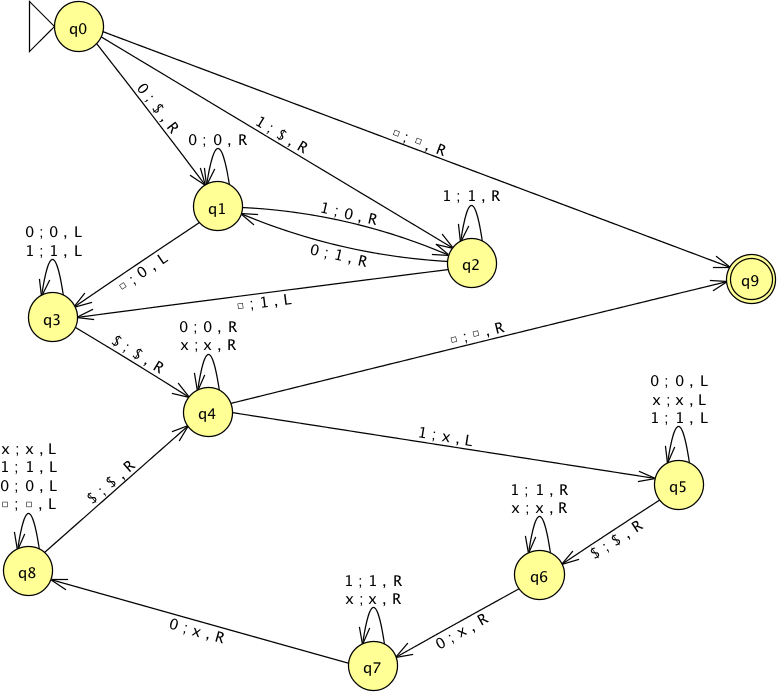
\includegraphics[scale=.6]{problem_2.png}
    \end{figure}
    Initially if the tape is blank accept, as zero $0$s is twice as many as zero $1$s. Otherwise, append a \$ onto the
    tape so the machine knows where the beginning of the tape is. It can then easily mark off pairs of 0s for each 1 it
    encounters. After each cycle, it rewinds the tape to the \$ so that it starts at the beginning.
  \end{solution}
\end{problem}

\begin{problem}{3}
  \begin{solution}
    Because we don't know the depth of the tree on input $s_i$ simply running the machine on each string is not safe
    because the machine may find itself running forever if there are any infinite loops. That is why the correct
    definition uses $i$ steps on each input, so that a single input doesn't prevent the rest of the strings from being
    enumerated.
  \end{solution}
\end{problem}

\begin{problem}{4}
  \begin{solution}
    The problem with this description is that it involves an infinite set. ``evaluate p on all of these settings'',
    requires infinite iteration, because the set of integers in this case is not bounded. So the machine would run
    forever, but step 3 asks us to reject if it doesn't evaluate to zero. It is not possible to build a machine that
    iterates over an infinite set in a finite amount of steps.  Therefore the description is not of a legitimate Turing
    machine.
  \end{solution}
\end{problem}

\begin{problem}{5}
  \begin{solution}

  \end{solution}
\end{problem}

\begin{problem}{6}
  \begin{solution}
    This problem asks us to show that this type of Turing machine recognizes the class of Turing-recognizable languages.
    So we need to show equivalence from both directions.
    \br
    A TM with an infinite tape in both directions is easy to show equivalence with a standard Turing Machine.  All that
    we need to do is add a special symbol to the beginning of the input symbols and have the doubly infinite Turing
    machine stop reading left when it encounters this special symbol.
    \br
    The other direction is more difficult, but can be done similarly.  We could use the k-tape Turing machine discussed
    in class, in this case with k set to 2.  One tape would represent symbols to the left, the other to the right. The
    input string would be on one tape, and when the head moves left of the first symbol on the tape the machine would
    switch to the second tape which would be blank. When the doubly infinite machine is instructed to move left, the
    head on this tape would move right.  Similarly when the doubly infinite machine is instructed to move right, the
    head would move left until it hit the bound, and then switch back to the other tape.
  \end{solution}
\end{problem}

\begin{problem}{7}
  \begin{solution}
    Because we can't move left, and don't know what is to the right, there is no way to maintain the functionality of
    the traditional Turing machine with this variant.  Further, this machine functionally describes a NFA, which we know
    to be functionally weaker than a TM. The machine can move forward, processing the input, but never backward on the
    string. Since there is no stack, there is no means of storing any of the inputs we have read. Once input is
    consumed, it cannot be recovered.
  \end{solution}
\end{problem}

\begin{problem}{8}
  \begin{solution}

  \end{solution}
\end{problem}

\end{document}
